\section{Auswertung}
\label{sec:Auswertung}
\subsection{Zeitabhänigkeit der Amplitude einer gedämpften Schwingung}
    Zeichnet man die Einhüllenden in den Druck der gedämpften Schwinung ein
    (s.unten), so kann man die Parameter der e- Funktion brechenen.
    \begin{figure}
      \centering
      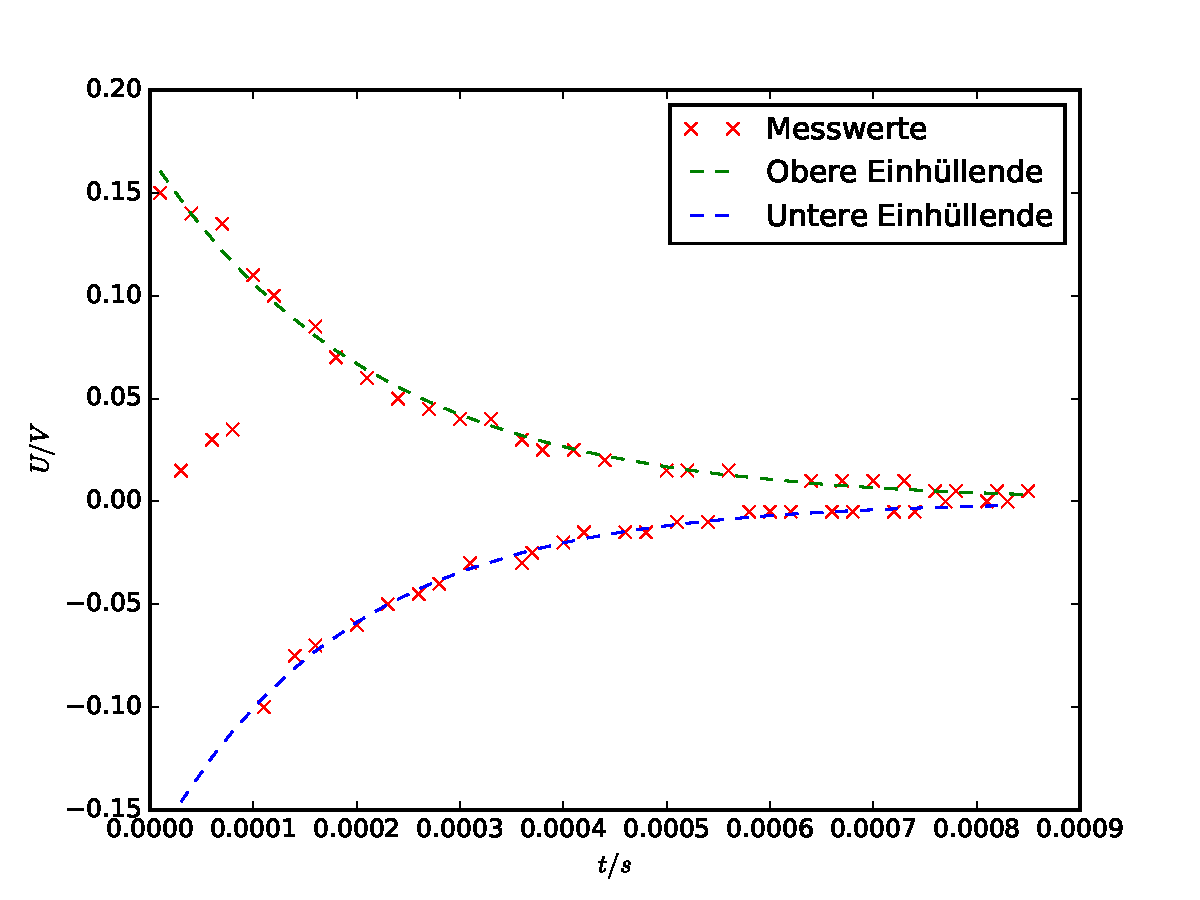
\includegraphics[width=\textwidth]{./logos/5aplot.pdf}
        \caption{Einhüllenden der Schwingungskurve}
        \label{fig:5aplot}
      \end{figure}
\FloatBarrier
    Dann ergibt sich für die obere Einhüllende das Wertepaar:
    $ A_0 = (0,16 \pm 0,003) \, \symup{V} $ und für $ \mu =  (732,99 \pm 20,8)\, \frac{1}{\symup{s}} $.
    Die untere Einhüllende ergibt sich dann das Wertepaar
    $ A_0 = (-0,17 \pm 0,005) \, \symup{V} $ und $ \mu =  (852,44 \pm 24,39) \, \frac{1}{\symup{s}} $.
    Der Mittelwert des oberen und unteren Widerstand ergibt:
    $ \mu = (793 \pm 16) \, \frac{1}{\symup{s}} $.
    Daraus ergibt sich für Abklingdauer:
    $T_{ex} = \frac{1}{2\pi\mu} = (0,002 \pm 4\cdot10^{-6}) \, \symup{s} $.
    Der effektiv Wiederstand liegt bei
    $ R_{eff} = (100,7 \pm 2,1) \, \si{Ohm} $.
    % Nun folgt die Abweichung von den Literaturwerten:
    % $ \increment T = 0,22\cdot10^{-3} \pm 0,4\cdot10^{-5} s $
    % und $ \increment R = 52,6 \pm 2,1 \si{Ohm}$
  \subsection{Aperodischer Grenzfall}
  \begin{figure}
    \centering
    \caption{Spannungen im Schwingkreis}
    \begin{subfigure}{0.48\textwidth}
      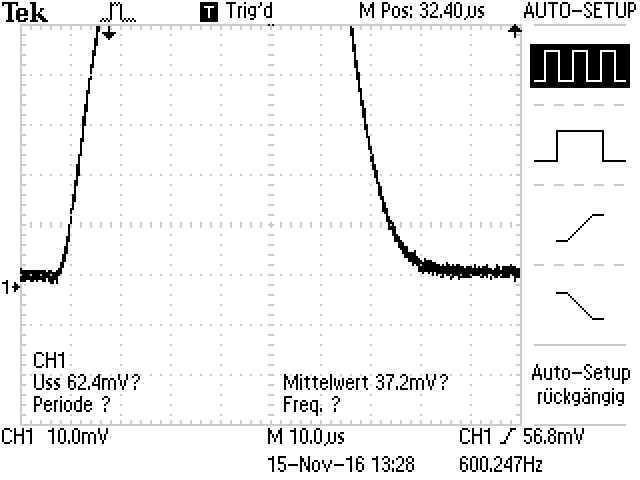
\includegraphics[height= 5cm]{./logos/5Print.JPG}
      \caption{bei einer Erregerfrequenz von 3,5 kHz}
      \label{fig:p1}
    \end{subfigure}
    \begin{subfigure}{0.48\textwidth}
      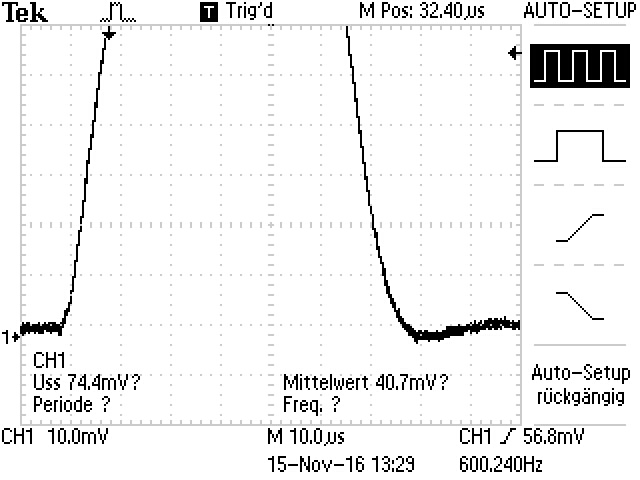
\includegraphics[height= 5cm]{./logos/6Print.JPG}
      \caption{bei einer Erregerfrequenz von 3 kHz}
      \label{fig:p2}
    \end{subfigure}
    \\
    \begin{subfigure}{0.48\textwidth}
      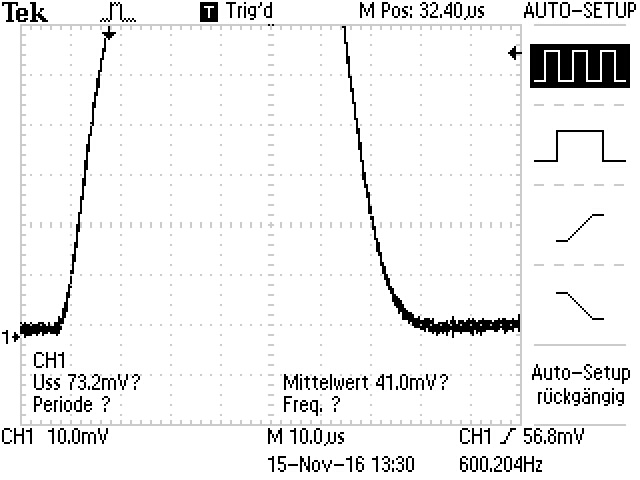
\includegraphics[height= 5cm]{./logos/7Print.JPG}
      \caption{bei einer Erregerfrequenz von 3,3 kHz}
      \label{fig:p3}
    \end{subfigure}
      \label{fig:prints}
  \end{figure}
  \FloatBarrier
      Das erste Bild (von oben nach unten) zeigt die Spannung im Schwingkreis
      bei einer Erregerfrequenz von 3,5 $kHz$.
      Das zweite Bild zeigt Die Spannung bei 3 kHz. Das dritte Bild zeigt die
      Spannung bei 3,3 kHz. Es ist zusehen das es einen Überschwung bei 3,5 kHz
      gibt und bei 3 kHz die Relaxion noch nicht
      ihr Maximum erreicht hat. Daraus folgt das der Widerstand $R_{ap}$ bei ca.
      3,3 kHz liegt. Der Literaturwert liegt bei
      $4390 \pm 9 \Omega$ .

  \subsection{Frequenzabhängigkeit der Kondensatorspannung}
  \begin{figure}
    \centering
    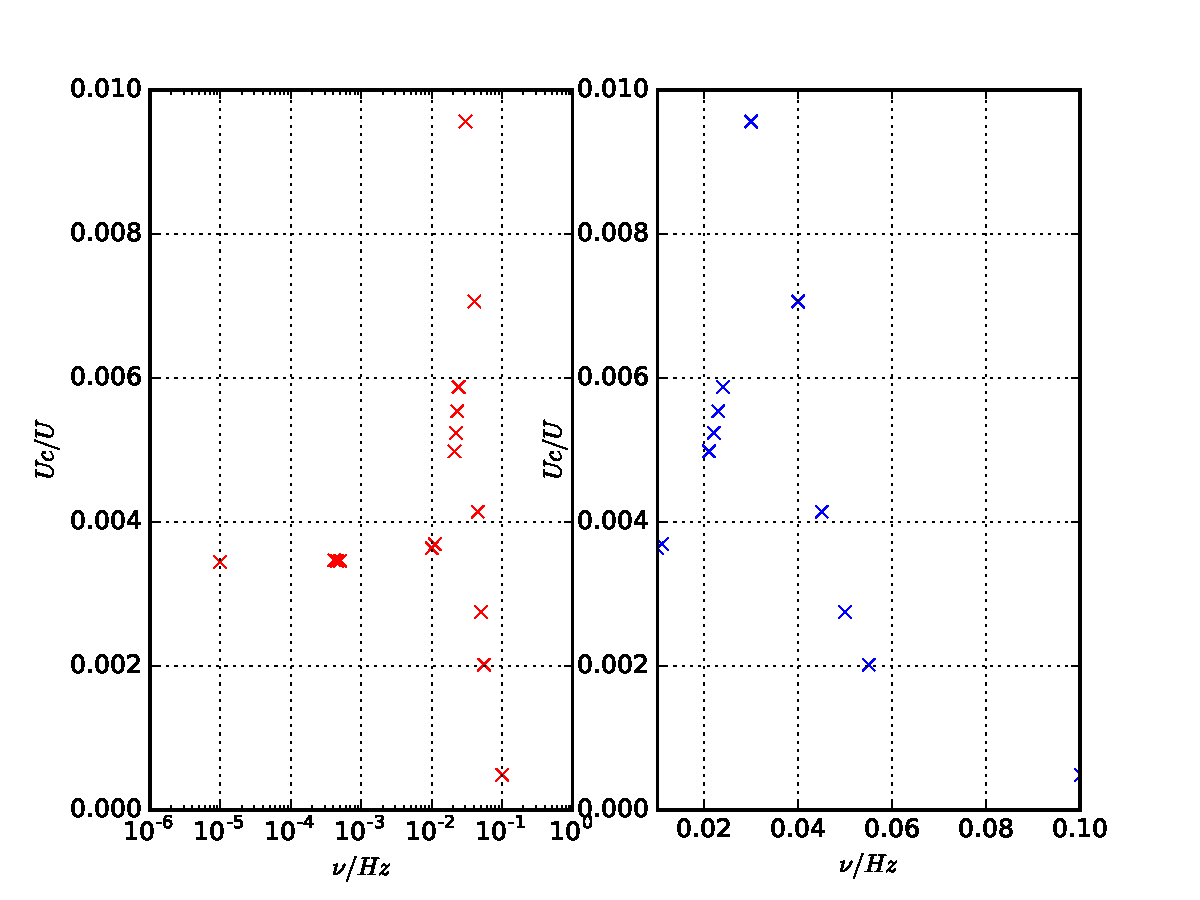
\includegraphics[width=\textwidth]{./logos/5cplot.pdf}
      \caption{Kondensatorspannung}
      \label{fig:5cplot}
    \end{figure}
    Für die Resonanzüberhöhung q ergibt sich experimentell: $q_{ex}= 2,34 $
    Theoretisch ergibt sich jedoch : $q_{theo}= 21,8  \pm 0,5 $
    Für den Frequenzen abstand ergibt sich eperimentell $ \nu_+ - \nu_- = 0,034 $
    und theoretisch $ \nu_{theo}= 137 \pm 2,9$
  \subsection{Frequenzabhängigikeit der Phase zwischen Erreger-und Kondensatorspannung}
  Die Frequenzabhängigkeit der Phase zwischen Erreger-und Kondensatorspannung
   lässt sich im Plot \ref{fig:5dplot} betrachten.
  Aufgrund zu weniger Daten können $\nu_+$ und $\nu_+$ , sowie $\nu_{res}$
  experimentel nicht eindeutig bestimmt werden.
  Die Erwartungswerte liegen aber für $\nu_{res}$ bei $(6,908 \pm 0,014)\cdot10^4$
  und für $\nu_+$ sowie $\nu_-$ bei
  $(3,536 \pm 0,007)\cdot10^4$ und $(3,377 \pm 0,007)\cdot10^4$
    \begin{figure}
      \centering
      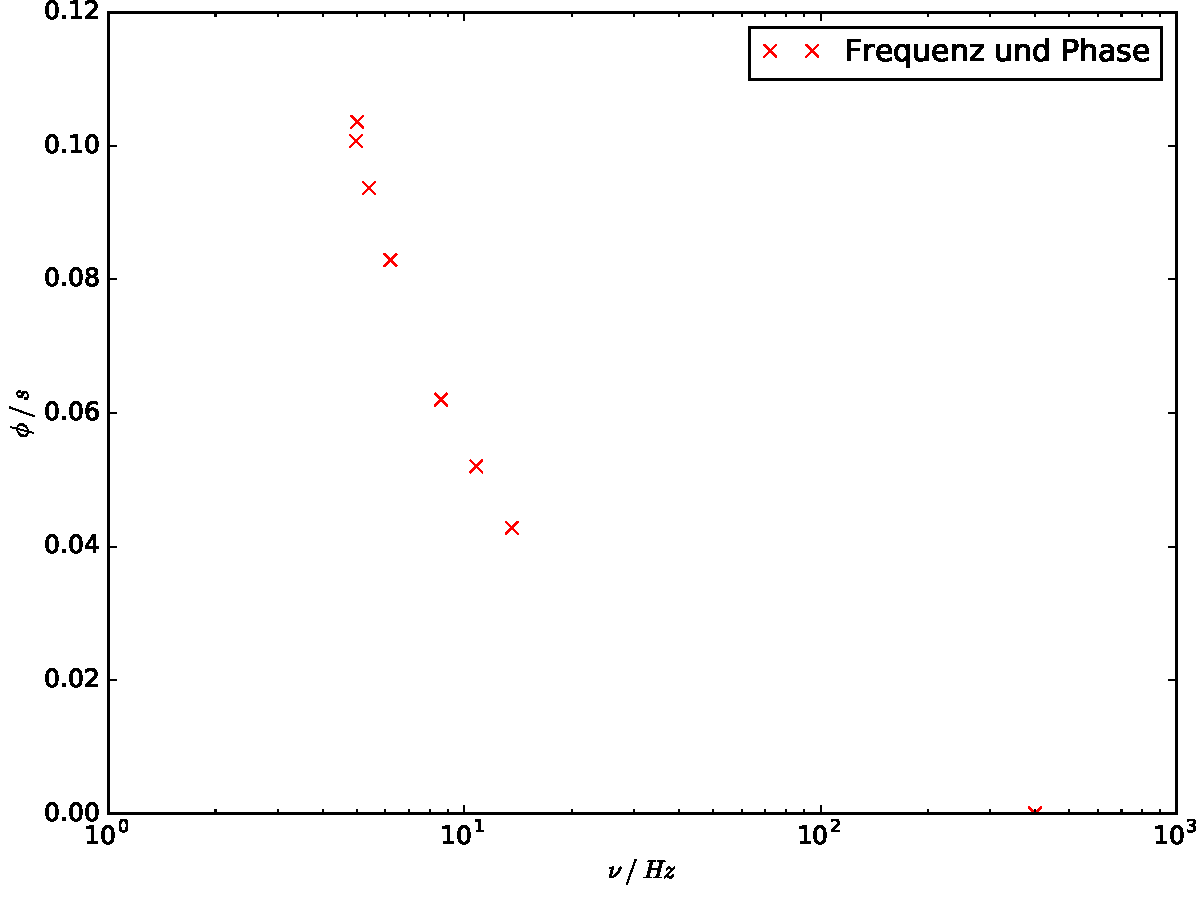
\includegraphics[width=\textwidth]{./logos/5dplot.pdf}
        \caption{Frequenzabhängigikeit der Phase zwischen Erreger-und Kondensatorspannung}
        \label{fig:5dplot}
      \end{figure}
    \subsection{Frequenzabhängigkeit des Scheinwiederstandes eines Serienkreises}
    \begin{figure}
      \centering
      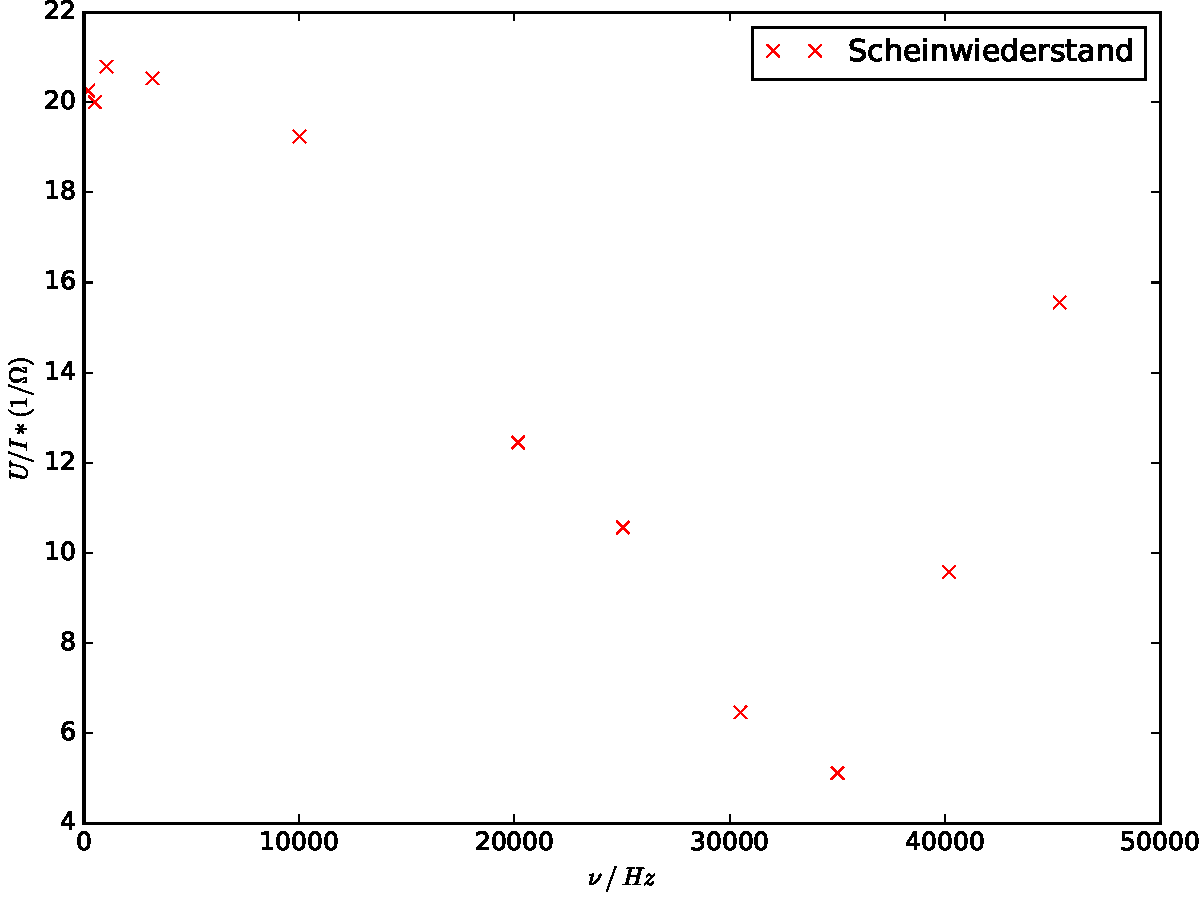
\includegraphics[width=\textwidth]{./logos/5eplot.pdf}
        \caption{Frequenzabhängigkeit des Scheinwiederstandes eines Serienkreises}
        \label{fig:5eplot}
      \end{figure}
      Der Plot\ref{fig:5eplot} zeigt den Abfall des Scheinwiederstandes bei
      steigender Frequenz. Jedoch steigt dieser
      wieder, dies steht im Wiederspruch zu unseren Erwartungen.
    \subsection{Werte von 3.1}
    Tab.\ref{tab:5a1tab},\ref{tab:5a2tab} und \ref{tab:5a3tab}
      \begin{table}
      \caption{Spannung und Frequenz der Gedämpften Schwingung 1}
      \label{tab:5a1tab}
      \sisetup{round-mode = places , round-precision = 2}
      \begin{tabular}{S S}
        \toprule
        {$U_i/mV$} & {$t/\mu s$ }\\
        \midrule
        1.500000000000000000e+02 & 1.000000000000000000e+01\\
        1.400000000000000000e+02 & 4.000000000000000000e+01\\
        1.350000000000000000e+02 & 7.000000000000000000e+01\\
        1.100000000000000000e+02 & 1.000000000000000000e+02\\
        1.000000000000000000e+02 & 1.200000000000000000e+02\\
  8.500000000000000000e+01 & 1.600000000000000000e+02\\
  7.000000000000000000e+01 & 1.800000000000000000e+02\\
  6.000000000000000000e+01 & 2.100000000000000000e+02\\
  5.000000000000000000e+01 & 2.400000000000000000e+02\\
  4.500000000000000000e+01 & 2.700000000000000000e+02\\
    4.000000000000000000e+01 & 3.000000000000000000e+02\\
  4.000000000000000000e+01 & 3.300000000000000000e+02\\
  3.000000000000000000e+01 & 3.600000000000000000e+02\\
  2.500000000000000000e+01 & 3.800000000000000000e+02\\
  2.500000000000000000e+01 & 4.100000000000000000e+02\\
  2.000000000000000000e+01 & 4.400000000000000000e+02\\
  1.500000000000000000e+01 & 5.000000000000000000e+02\\
  1.500000000000000000e+01 & 5.200000000000000000e+02\\
  1.500000000000000000e+01 & 5.600000000000000000e+02\\
  1.000000000000000000e+01 & 6.400000000000000000e+02\\
  1.000000000000000000e+01 & 6.700000000000000000e+02\\
  1.000000000000000000e+01 & 7.000000000000000000e+02\\
  1.000000000000000000e+01 & 7.300000000000000000e+02\\
  5.000000000000000000e+00 & 7.600000000000000000e+02\\
  5.000000000000000000e+00 & 7.800000000000000000e+02\\
  5.000000000000000000e+00 & 8.200000000000000000e+02\\
  5.000000000000000000e+00 & 8.500000000000000000e+02\\
  1.500000000000000000e+01 & 3.000000000000000000e+01\\
  3.000000000000000000e+01 & 6.000000000000000000e+01\\
  3.500000000000000000e+01 & 8.000000000000000000e+01\\
  -1.000000000000000000e+02 & 1.100000000000000000e+02\\
  -7.500000000000000000e+01 & 1.400000000000000000e+02\\
  -7.000000000000000000e+01 & 1.600000000000000000e+02\\
  -6.000000000000000000e+01 & 2.000000000000000000e+02\\
  -5.000000000000000000e+01 & 2.300000000000000000e+02\\
  -4.500000000000000000e+01 & 2.600000000000000000e+02\\
  -4.000000000000000000e+01 & 2.800000000000000000e+02\\
  -3.000000000000000000e+01 & 3.100000000000000000e+02\\
  -3.000000000000000000e+01 & 3.600000000000000000e+02\\
  -2.500000000000000000e+01 & 3.700000000000000000e+02\\
  \bottomrule
\end{tabular}
\end{table}
\begin{table}
\caption{Spannung und Frequenz der Gedämpften Schwingung 2}
\label{tab:5a2tab}
\sisetup{round-mode = places , round-precision = 2}
\begin{tabular}{S S}
  \toprule
  {$U_i/mV$} & {$t/\mu s$ }\\
  \midrule
  -2.000000000000000000e+01 & 4.000000000000000000e+02\\
  -1.500000000000000000e+01 & 4.200000000000000000e+02\\
  -1.500000000000000000e+01 & 4.600000000000000000e+02\\
  -1.500000000000000000e+01 & 4.800000000000000000e+02\\
  -1.000000000000000000e+01 & 5.100000000000000000e+02\\
  -1.000000000000000000e+01 & 5.400000000000000000e+02\\
  -5.000000000000000000e+00 & 5.800000000000000000e+02\\
  -5.000000000000000000e+00 & 6.000000000000000000e+02\\
  -5.000000000000000000e+00 & 6.200000000000000000e+02\\
  -5.000000000000000000e+00 & 6.600000000000000000e+02\\
    4.000000000000000000e+01 & 3.000000000000000000e+02\\
4.000000000000000000e+01 & 3.300000000000000000e+02\\
3.000000000000000000e+01 & 3.600000000000000000e+02\\
2.500000000000000000e+01 & 3.800000000000000000e+02\\
2.500000000000000000e+01 & 4.100000000000000000e+02\\
2.000000000000000000e+01 & 4.400000000000000000e+02\\
1.500000000000000000e+01 & 5.000000000000000000e+02\\
1.500000000000000000e+01 & 5.200000000000000000e+02\\
1.500000000000000000e+01 & 5.600000000000000000e+02\\
1.000000000000000000e+01 & 6.400000000000000000e+02\\
1.000000000000000000e+01 & 6.700000000000000000e+02\\
1.000000000000000000e+01 & 7.000000000000000000e+02\\
1.000000000000000000e+01 & 7.300000000000000000e+02\\
5.000000000000000000e+00 & 7.600000000000000000e+02\\
5.000000000000000000e+00 & 7.800000000000000000e+02\\
5.000000000000000000e+00 & 8.200000000000000000e+02\\
5.000000000000000000e+00 & 8.500000000000000000e+02\\
1.500000000000000000e+01 & 3.000000000000000000e+01\\
3.000000000000000000e+01 & 6.000000000000000000e+01\\
3.500000000000000000e+01 & 8.000000000000000000e+01\\
-1.000000000000000000e+02 & 1.100000000000000000e+02\\
-7.500000000000000000e+01 & 1.400000000000000000e+02\\
-7.000000000000000000e+01 & 1.600000000000000000e+02\\
-6.000000000000000000e+01 & 2.000000000000000000e+02\\
\bottomrule
\end{tabular}
\end{table}
\begin{table}
\caption{Spannung und Frequenz der Gedämpften Schwingung 3}
\label{tab:5a3tab}
\sisetup{round-mode = places , round-precision = 2}
\begin{tabular}{S S}
\toprule
{$U_i/mV$} & {$t/\mu s$ }\\
\midrule
-5.000000000000000000e+01 & 2.300000000000000000e+02\\
-4.500000000000000000e+01 & 2.600000000000000000e+02\\
-4.000000000000000000e+01 & 2.800000000000000000e+02\\
-3.000000000000000000e+01 & 3.100000000000000000e+02\\
-3.000000000000000000e+01 & 3.600000000000000000e+02\\
-2.500000000000000000e+01 & 3.700000000000000000e+02\\
-2.000000000000000000e+01 & 4.000000000000000000e+02\\
-1.500000000000000000e+01 & 4.200000000000000000e+02\\
-1.500000000000000000e+01 & 4.600000000000000000e+02\\
-1.500000000000000000e+01 & 4.800000000000000000e+02\\
-1.000000000000000000e+01 & 5.100000000000000000e+02\\
-1.000000000000000000e+01 & 5.400000000000000000e+02\\
-5.000000000000000000e+00 & 5.800000000000000000e+02\\
-5.000000000000000000e+00 & 6.000000000000000000e+02\\
-5.000000000000000000e+00 & 6.200000000000000000e+02\\
-5.000000000000000000e+00 & 6.600000000000000000e+02\\
-5.000000000000000000e+00 & 6.800000000000000000e+02\\
-5.000000000000000000e+00 & 7.200000000000000000e+02\\
-5.000000000000000000e+00 & 7.400000000000000000e+02\\
0.000000000000000000e+00 & 7.700000000000000000e+02\\
0.000000000000000000e+00 & 8.100000000000000000e+02\\
0.000000000000000000e+00 & 8.300000000000000000e+02\\
-5.000000000000000000e+00 & 6.800000000000000000e+02\\
  -5.000000000000000000e+00 & 7.200000000000000000e+02\\
  -5.000000000000000000e+00 & 7.400000000000000000e+02\\
  0.000000000000000000e+00 & 7.700000000000000000e+02\\
  0.000000000000000000e+00 & 8.100000000000000000e+02\\
  0.000000000000000000e+00 & 8.300000000000000000e+02\\
  \bottomrule
\end{tabular}
\end{table}
\subsection{Werte von 3.3}
Tab.\ref{tab:5ctab}
\begin{table}
  \centering
  \caption{Spannung und Frequenzabhängigkeit der Kondensatorspannung}
  \label{tab:5ctab}
  \sisetup{round-mode = places , round-precision = 2}
\begin{tabular}{S S S}
  \toprule
  $U_{ss}/mV$ & $U_{eff}/mV$ & $t/\mu s$ \\
  \midrule
  1.560000000000000000e+02 & 5.550000000000000000e+01 & 4.150000000000000000e+02\\
  1.560000000000000000e+02 & 5.539999999999999858e+01 & 4.500000000000000000e+02\\
  1.560000000000000000e+02 & 5.539999999999999858e+01 & 5.000000000000000000e+02\\
  1.680000000000000000e+02 & 5.820000000000000284e+01 & 1.000000000000000000e+04\\
  1.720000000000000000e+02 & 5.910000000000000142e+01 & 1.100000000000000000e+04\\
  2.220000000000000000e+02 & 7.720000000000000284e+01 & 2.000000000000000000e+04\\
  2.720000000000000000e+02 & 9.400000000000000000e+01 & 2.400000000000000000e+04\\
  2.560000000000000000e+02 & 8.859999999999999432e+01 & 2.300000000000000000e+04\\
  2.440000000000000000e+02 & 8.379999999999999716e+01 & 2.200000000000000000e+04\\
  2.340000000000000000e+02 & 7.970000000000000284e+01 & 2.100000000000000000e+04\\
  4.480000000000000000e+02 & 1.530000000000000000e+02 & 3.000000000000000000e+04\\
  3.240000000000000000e+02 & 1.130000000000000000e+02 & 4.000000000000000000e+04\\
  1.960000000000000000e+02 & 6.629999999999999716e+01 & 4.500000000000000000e+04\\
  1.260000000000000000e+02 & 4.400000000000000000e+01 & 5.000000000000000000e+04\\
  9.440000000000000568e+01 & 3.229999999999999716e+01 & 5.500000000000000000e+04\\
  1.560000000000000000e+02 & 5.510000000000000142e+01 & 9.810000000000000497e+00\\
  2.139999999999999858e+01 & 7.799999999999999822e+00 & 1.002000000000000000e+05\\

  \bottomrule
\end{tabular}

\end{table}
\subsection{Werte von 3.4}
Tab.\ref{tab:5dtab}
\begin{table}
  \centering
  \caption{Frequenzabhängigkeit der Phase zwischen Erreger-und Kondensatorspannung}
  \label{tab:5dtab}
  \sisetup{round-mode = places , round-precision = 2}
\begin{tabular}{S S}
  \toprule
  $\nu/Hz$ &  $\frac{\phi}{\mu s}$ \\
  \midrule
  1.007000000000000000e+05 & 4.959999999999999964e+00\\
  2.323000000000000000e+03 & 0.000000000000000000e+00\\
  4.282000000000000000e+04 & 1.359999999999999964e+01\\
  5.200000000000000000e+04 & 1.080000000000000071e+01\\
  6.200000000000000000e+04 & 8.599999999999999645e+00\\
  8.290000000000000000e+04 & 6.200000000000000178e+00\\
  9.370000000000000000e+04 & 5.400000000000000355e+00\\
  1.036000000000000000e+05 & 5.000000000000000000e+00\\
  4.156000000000000227e+01 & 4.000000000000000000e+02\\
  5.500000000000000000e+01 & 4.000000000000000000e+02\\
  5.008000000000000114e+02 & 0.000000000000000000e+00\\
  1.985000000000000000e+02 & 0.000000000000000000e+00\\

  \bottomrule
\end{tabular}

\end{table}
\subsection{Werte von 3.5}
Tab.\ref{tab:5etab}
\begin{table}
  \centering
  \caption{Frequenzabhängigkeit des Scheinwiederstandes}
  \label{tab:5etab}
  \sisetup{round-mode = places , round-precision = 2}
\begin{tabular}{S S S}
  \toprule
  $U_{pp}/V$ & $ I_{pp}/A$ &  $\nu/Hz$ \\
  \midrule
  3.119999999999999929e+01 & 1.540000000000000036e+00 & 1.985000000000000000e+02\\
  3.119999999999999929e+01 & 1.560000000000000053e+00 & 5.108999999999999773e+02\\
  3.160000000000000142e+01 & 1.520000000000000018e+00 & 1.046000000000000000e+03\\
  3.080000000000000071e+01 & 1.500000000000000000e+00 & 3.185000000000000000e+03\\
  3.039999999999999858e+01 & 1.580000000000000071e+00 & 1.001000000000000000e+04\\
  3.000000000000000000e+01 & 2.410000000000000142e+00 & 2.017000000000000000e+04\\
  3.000000000000000000e+01 & 2.839999999999999858e+00 & 2.504000000000000000e+04\\
  2.919999999999999929e+01 & 4.519999999999999574e+00 & 3.050000000000000000e+04\\
  2.800000000000000000e+01 & 5.480000000000000426e+00 & 3.501000000000000000e+04\\
  2.919999999999999929e+01 & 3.049999999999999822e+00 & 4.019000000000000000e+04\\
  3.080000000000000071e+01 & 1.979999999999999982e+00 & 4.533000000000000000e+04\\
  \bottomrule
\end{tabular}

\end{table}
